%CLASSE DO DOCUMENTO

\documentclass[12pt,a4paper]{book}

%SUPORTES PARA O DOCUMENTO

\usepackage[utf8]{inputenc} % Codificação de entrada
\usepackage[T1]{fontenc} % Codificação da fonte
\usepackage[brazil]{babel} % Suporte ao português do Brasil

\usepackage{geometry} % Para configurar margens
\usepackage{graphicx} % Para inserir figuras
\usepackage{float}
\usepackage{siunitx}
\usepackage{tcolorbox}
\usepackage{listings}
\lstset{
    extendedchars=true,
    literate=
    {á}{{\'a}}1 {é}{{\'e}}1 {í}{{\'i}}1 {ó}{{\'o}}1 {ú}{{\'u}}1
    {Á}{{\'A}}1 {É}{{\'E}}1 {Í}{{\'I}}1 {Ó}{{\'O}}1 {Ú}{{\'U}}1
    {à}{{\`a}}1 {è}{{\`e}}1 {ì}{{\`i}}1 {ò}{{\`o}}1 {ù}{{\`u}}1
    {À}{{\`A}}1 {È}{{\'E}}1 {Ì}{{\`I}}1 {Ò}{{\`O}}1 {Ù}{{\`U}}1
    {ã}{{\~a}}1 {ẽ}{{\~e}}1 {ĩ}{{\~i}}1 {õ}{{\~o}}1 {ũ}{{\~u}}1
    {Ã}{{\~A}}1 {Ẽ}{{\~E}}1 {Ĩ}{{\~I}}1 {Õ}{{\~O}}1 {Ũ}{{\~U}}1
    {â}{{\^a}}1 {ê}{{\^e}}1 {î}{{\^i}}1 {ô}{{\^o}}1 {û}{{\^u}}1
    {Â}{{\^A}}1 {Ê}{{\^E}}1 {Î}{{\^I}}1 {Ô}{{\^O}}1 {Û}{{\^U}}1
    {ç}{{\c c}}1 {Ç}{{\c C}}1
}
\usepackage{xcolor}
\tcbuselibrary{skins, breakable}
\usepackage[colorlinks=true, linkcolor=blue, urlcolor=blue]{hyperref} %hiperlink
\usepackage{amsmath, amssymb} % Suporte matemático avançado
\usepackage{enumitem}
\setlist{  
  topsep=2pt,    % Espaço antes/depois da lista
  itemsep=1pt,   % Espaço entre itens
  parsep=0pt     % Espaço dentro do item
}
\lstset{
    basicstyle=\ttfamily\small,
    breaklines=true,
    frame=single,
    numbers=left,
    numberstyle=\tiny\color{gray},
    keywordstyle=\color{blue}\bfseries,
    commentstyle=\color{green!50!black},
    stringstyle=\color{red},
    showstringspaces=false,
    tabsize=4,
    language=C,
    morekeywords={pragma, config, TRISA, PORTA, PORTAbits}
}

%CAPA
\title{Microcontroladores - Vol. 1}
\author{Gabriel Duarte Marques}
\date{Março 2025}

%CONFIG DE INICIO DO DOC
\begin{document}
\maketitle
\tableofcontents

% ESCRITA do DOC
\chapter{Introdução aos Microcontroladores}
\section{O que são Microcontroladores}
Nesse momento é pressuposto que em algum momento você já ouviu ou utilizou o Arduíno, a famosa placa azul é geralmente a porta de entrada para o mundo da eletrônica e por exemplo no modelo UNO da marca temos soldado na placa um microcontrolador de modelo ATmega328P e além dele existem outros componentes que fazem o Arduíno funcionar e facilitar a montagem de circuitos.\par
Assim como o microcontrolador usado no Arduíno temos de outras fabricantes seus próprios modelos de microcontroladores a Microchip tem os PIC e suas respectivas famílias e a Intel tem os 8051 e famílias, cada fabricante, cada modelo, tem suas características por isso se deve ao utilizar qualquer componente eletrônico que seja se faz necessário ao menos ler por cima o \textbf{datasheet} que é um documento criado pelo fabricante que resume o desempenho e outras características técnicas de um produto e que fornece detalhes suficientes para que possa ser usado.\par
Definido como se parecem e de onde vieram, os \textbf{Microcontroladores} são pequenos computadores que estão por toda a parte no nosso cotidiano e note a seguir as nuâncias de \textbf{Controle} dele que vão desde os objetos mais simples como micro-ondas, ar-condicionados, controles remotos aos mais complexos como carros, aviões, equipamentos médicos e entre outros pois as implementações são infinitas, principalmente com o advento das IA's, diferente de um computador pessoal que se precisa de várias peças para funcionar, como processador, placa-mãe, disco rígido, fonte e outros, os microcontroladores contém todas esses componentes em um único chip e tendo um consumo energético menor se comparado ao seu irmão maior. \par
Com base na descrição e nos exemplos anteriores podemos então inferir que a palavra "Micro" pode significar pequeno e "Controlador" pode significar controle de processos então o conjunto \textbf{MicroControlador} pode significar pequeno controlador de processos.
\newpage
\section{Microcontroladores versus Microprocessadores}
Os Microcontroladores e Microprocessadores antes da década de 90 já existiam, mas foi durante essa época que com o avanço da miniaturização, o avanço das técnicas de processamento de silício e a fabricação de chips resultaram na capacidade de colocar cada vez mais transistores em um único núcleo, foram ganhando cada vez mais espaço e começaram a ser amplamente adotados em bens de consumo e sistemas de controle. Um microprocessador é essencialmente um processador de um computador em escala de menor tamanho, logo, ele necessita de todos os componentes que um computador também precisa para o seu funcionamento.
\par
Os microcontroladores por outro lado contém tudo que se necessita para o controle de sistemas em um único \textbf{CI} (Circuito Integrado) com memórias embutidas, conversores e entre outros componentes.
\section{Componentes Básicos de um Microcontrolador}
\begin{itemize}
    \item \textbf{Unidade central de processamento (CPU):} é o "cérebro" do computador, a CPU serve como o responsável pela execução de instruções e controle de operações.
    \item \textbf{Memória:} os microcontroladores contêm memória volátil a chamada \textbf{RAM} que armazena dados temporários para execução e memória flash não volátil (um tipo avançado de \textbf{EEPROM}) que armazena a memória de programa.
    \item \textbf{Periféricos:} um microcontrolador pode conter vários componentes auxiliares, como interfaces de entrada/saída (E/S) e isso incui uma infinidade de componentes aqui estão alguns deles temporizadores, contadores, conversores de sinal, módulos e entre outros.
\end{itemize}
\section{Tipos de Microcontroladores}
Os microcontroladores podem ser classificados de diversas formas, sendo as mais comuns baseadas em sua arquitetura, desempenho, tamanho da palavra e aplicação. Conhecer estas classificações é importante para a seleção adequada do dispositivo para cada projeto.
\newpage
\subsection{Classificação por Tamanho da Palavra}
Os microcontroladores podem ser classificados de acordo com o tamanho de dados que processam:
\begin{itemize}
    \item \textbf{8 bits:} São os mais comuns para aplicações de controle simples, como eletrodomésticos e brinquedos. Exemplos: AVR (Arduino), PIC16, 8051.
    \item \textbf{16 bits:} Oferecem maior poder de processamento para aplicações intermediárias. Exemplos: PIC24, MSP430.
    \item \textbf{32 bits:} Para aplicações que exigem maior capacidade de processamento e recursos. Exemplos: ARM Cortex-M, PIC32, ESP32.
    \item \textbf{64 bits:} Encontrados em aplicações embarcadas de alto desempenho.
\end{itemize}
\subsection{Plataformas Alternativas}
Além dos microcontroladores tradicionais, é importante mencionar os \textbf{FPGAs} (Field Programmable Gate Arrays) como uma plataforma alternativa para implementação de arquiteturas de microcontroladores. Embora os \textbf{FPGAs} não sejam microcontroladores, eles oferecem a flexibilidade de implementar arquiteturas personalizadas de microcontroladores em hardware reconfigurável.
\par Também temos os \textbf{CLPs (Controlador Lógico Programável):} Sistemas industriais modulares que incorporam microcontroladores em sua CPU. São projetados para ambientes industriais severos, resistência a vibrações, a poeira, a umidade e interferências eletromagnéticas, mas possuem custo elevado comparado a soluções baseadas em microcontroladores puros.
\subsection{Classificação por Família/Fabricante}
Existem diversos fabricantes no mercado, cada um com suas próprias famílias de microcontroladores:
\begin{itemize}
    \item \textbf{Microchip:} Famílias PIC (PIC10, PIC12, PIC16, PIC18, PIC24, PIC32)
    \item \textbf{Atmel:} Famílias AVR (utilizados no Arduino), megaAVR, tinyAVR
    \item \textbf{Texas Instruments:} MSP430, C2000, Tiva
    \item \textbf{STMicroelectronics:} STM8, STM32 (baseados em ARM)
    \item \textbf{NXP:} S08, Kinetis, LPC (baseados em ARM)
    \item \textbf{Espressif:} ESP8266, ESP32 (populares para IoT)
    \item \textbf{Intel:} 8051 e suas derivações
\end{itemize}

\subsection{Classificação por Arquitetura}
Os microcontroladores podem ser classificados conforme a arquitetura de seu conjunto de instruções:

\begin{itemize}
    \item \textbf{CISC (Complex Instruction Set Computer):} Utiliza um conjunto de instruções complexo e extenso, capaz de executar operações elaboradas com uma única instrução um exemplo de microcontroladores com arquitetura CISC é os da família 8051 da Intel.
    \item \textbf{RISC (Reduced Instruction Set Computer):} Emprega um conjunto reduzido de instruções simples e otimizadas um exemplo de microcontroladores com arquitetura RISC são os baseados em ARM.
\end{itemize}
\chapter{Arquitetura dos Microcontroladores}
\section{Arquiteturas Fundamentais}
\subsection{Arquitetura Harvard}
Desenvolvida originalmente na Universidade de Harvard em 1944, esse tipo de arquitetura é caracterizada pela separação física das memórias de programa e dados, com barramentos independentes para cada uma. Este tipo de projeto permite acesso simultâneo às duas memórias, aumentando a eficiência em aplicações de tempo real.
\begin{figure}[h]
  \centering
  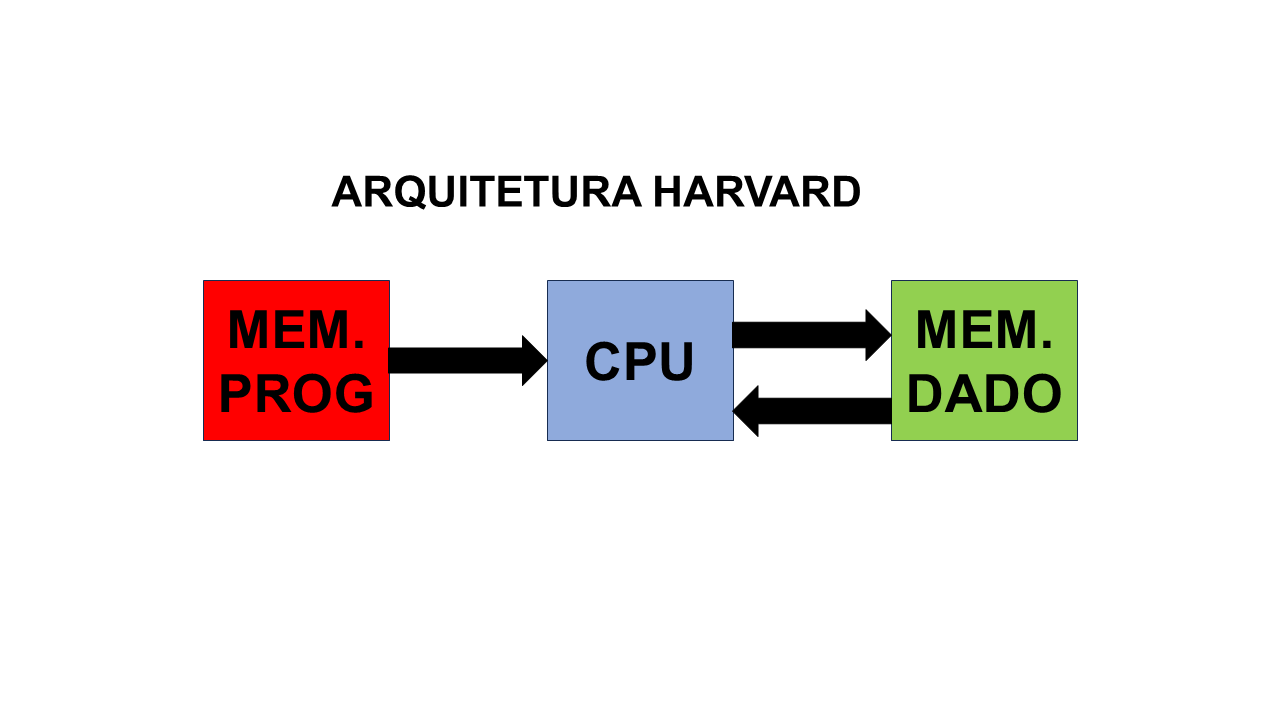
\includegraphics[width=0.9\textwidth]{imgs/cap_2/arq_harv.png}
  \caption{Diagrama da arquitetura Harvard}
  \label{fig:harvard}
\end{figure}

\subsection{Arquitetura von Neumann}  
Proposta por John von Neumann em 1945, unifica programas e dados em um único barramento e espaço de memória, simplificando o projeto, mas essa arquitetura cria o \textbf{gargalo de von Neumann}, onde a CPU não pode buscar instruções e dados simultaneamente.
Nos computadores modernos, o gargalo é mitigado por:  
\begin{itemize}  
    \item \textbf{Caches L1 separadas:} Adoção de arquitetura \textit{Harvard modificada} com L1i (instruções) e L1d (dados) para acesso paralelo.
    \item \textbf{Técnicas de paralelismo:} Pipelining, execução fora de ordem e multithreading.
    \item \textbf{Memória unificada superior:} Caches L2/L3 e RAM mantêm o modelo von Neumann.  
\end{itemize}

\begin{figure}[h]
  \centering
  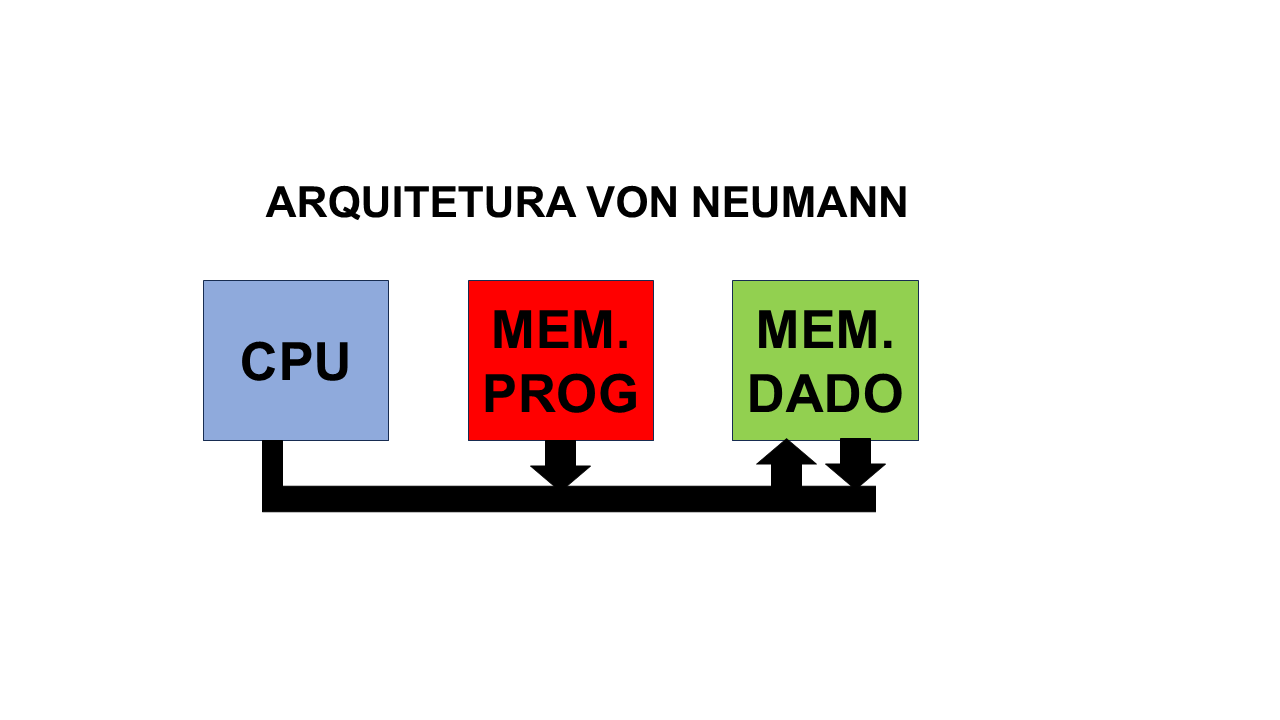
\includegraphics[width=0.9\textwidth]{imgs/cap_2/arq_neumann.png}
  \caption{Diagrama da arquitetura Von Neumann}
  \label{fig:neumann}
\end{figure}
\newpage
\subsection{Comparação entre Harvard e Von Neumann}
As arquiteturas Harvard e Von Neumann são fundamentais no design de microcontroladores e microprocessadores, cada uma com suas características distintas e aplicações específicas.
Observando as figuras anteriores \ref{fig:harvard} e \ref{fig:neumann} é possível ver que para sair de uma arquitetura Harvard para uma de Von Neumann é necessário somente uma porta lógica \textbf{AND} que sirva de junção para as memórias de programa e de dados, agora o exercício contrário não é simples de se perceber.
\par A seguir uma tabela que exemplifica as diferenças entre as duas arquiteturas fundamentais:
\begin{table}[H]
  \centering
  \begin{tabular}{|l|c|c|}
    \hline
    \textbf{Característica} & \textbf{Harvard} & \textbf{Von Neumann} \\
    \hline
    Barramentos & Separados & Único \\
    Segurança & Maior & Menor \\
    Custo & Maior & Menor \\
    Aplicação & Sistemas Embarcados & Computação geral \\
    \hline
  \end{tabular}
  \caption{Comparação entre as arquiteturas}
  \label{tab:arq_comparacao}
\end{table}
\section{Componentes Básicos da Arquitetura}
A arquitetura básica de um microcontrolador é composta por componentes interconectados que trabalham em conjunto para executar tarefas de controle. A Figura \ref{fig:arq_bas} ilustra a organização típica desses componentes:
\begin{figure}[h]
  \centering
  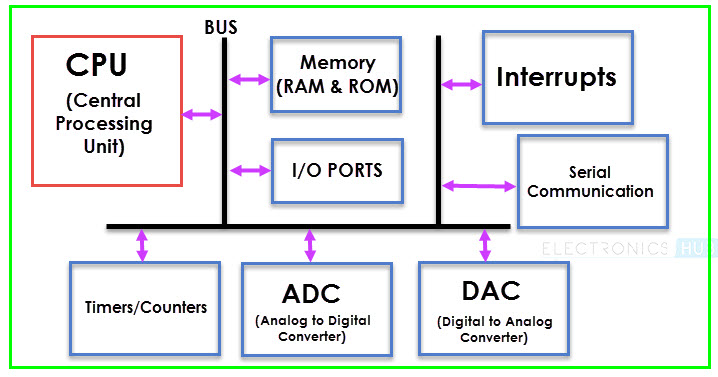
\includegraphics[width=0.9\textwidth]{imgs/cap_2/arq_basica.jpeg}
  \caption{Arquitetura Básica}
  \label{fig:arq_bas}
\end{figure}
\par
Os principais componentes e suas funções são:

\begin{itemize}
\item \textbf{CPU (Unidade Central de Processamento)}: Executa instruções armazenadas na memória de programa, controlando o fluxo de dados entre os componentes. Em microcontroladores RISC, opera com um conjunto reduzido de instruções otimizadas.

\item \textbf{Memória de Programa (Flash/EEPROM)}: Armazena o código-fonte do firmware de forma não volátil. Em um Arduino Uno, por exemplo, possui 32 KB para armazenar instruções.

\item \textbf{Memória de Dados (RAM)}: Armazena variáveis temporárias durante a execução do programa. Possui acesso rápido, mas é volátil (perde dados ao desligar).

\item \textbf{Barramento de Sistema}: Conjunto de linhas de comunicação que interconectam CPU, memória e periféricos. Inclui:
\begin{itemize}
\item Barramento de dados (transfere instruções/dados)
\item Barramento de endereços (localiza memória/periféricos)
\item Barramento de controle (sincroniza operações)
\end{itemize}

\item \textbf{Periféricos}: Circuitos especializados para funções específicas:
\begin{itemize}
\item Temporizadores/Contadores (ex: TIMER0 no PIC16F877A)
\item Conversores Analógico-Digital (ADC)
\item Módulos de comunicação (UART, SPI, I2C)
\item Portas GPIO (General Purpose Input/Output)
\end{itemize}
\item \textbf{Interface de E/S}: Conecta o microcontrolador a sensores, atuadores e outros dispositivos externos.
\end{itemize}
\chapter{PICs: Fundamentos Teóricos}
\section{Visão Geral da Família PIC}
São microcontroladores de arquitetura PIC (Peripheral Interface Controller) da Microchip Technology e passou por uma evolução significativa desde seu surgimento em 1975. Sua trajetória reflete as demandas tecnológicas de cada era, com adaptações que mantêm compatibilidade retroativa em algumas famílias e rupturas em outras.
\subsection{Relações Intra-Familiares}
As famílias de microcontroladores PIC são projetadas com uma filosofia de \textit{hardware modular}, onde modelos da mesma série compartilham características fundamentais, variando apenas em aspectos específicos como memória, portas e pequenas diferenças na programação para atender diferentes nichos de aplicação. Por exemplo, os PICs de modelo \textbf{16F628A} compartilham a mesma família que os modelos \textbf{16F627A}, \textbf{16F648A} e compartilham o mesmo \textit{\textbf{datasheet}}.
\subsection{Formatos Físicos ou Encapsulamento}
\begin{itemize}
\item \textbf{DIP/PTH (Dual In-line Package):}
  \begin{itemize}
  \item Pinos paralelos em duas fileiras
  \item 6 a 40 pinos - DIP40,DIP6...
  \item Fácil soldagem
  \end{itemize}
  
\item \textbf{SMD (Surface-Mount Device):}
  \begin{itemize}
  \item Montagem direta na superfície
  \item Tipos comuns: SOIC, QFN, MLF
  \item Compacta
  \item Uso de difíceis técnicas de soldagem
  \end{itemize}
\end{itemize}

\begin{figure}[H]
  \centering
  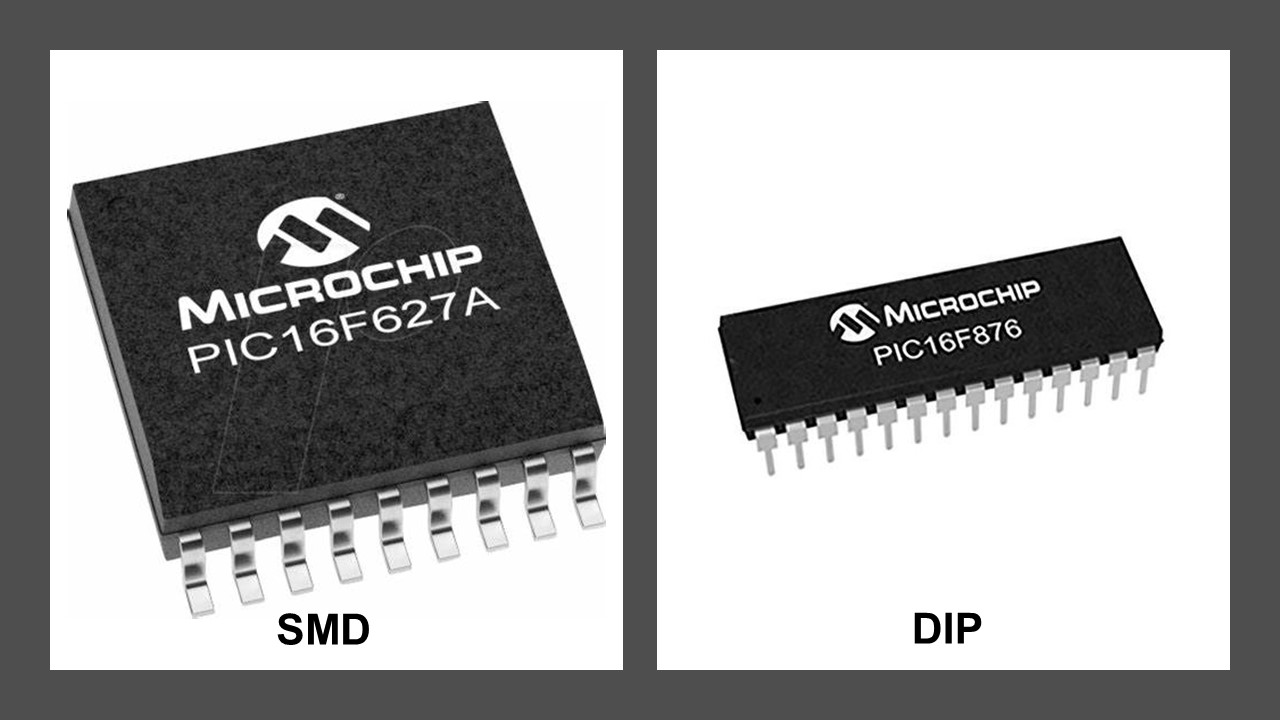
\includegraphics[width=0.6\textwidth]{imgs/cap_3/DIP_SMD.jpg}
  \caption{Diferença do Chip DIP e SMD}
  \label{fig:smd_dip}
\end{figure}
\subsection{Famílias Principais}
\begin{itemize}
    \item \textbf{PIC10/12/16 (8-bit):} Compartilham várias semelhanças em sua arquitetura e conjunto de instruções, o que permite que o código seja facilmente portado entre si com pequenas modificações:
\end{itemize}
\begin{itemize}
    \item \textbf{PIC18 (Enhanced 8-bit):} Tem um conjunto de instruções expandido,pilha e tamanho de bits maior com recursos de programação mais avançados.
\end{itemize}
\begin{itemize}
    \item \textbf{PIC24/33 (16-bit):} Permitem operações mais complexas, pode ter interface gráfica integrada e oferece suporte nativo a protocolos \textbf{CAN} e \textbf{USB}.
\end{itemize}
\begin{itemize}
    \item \textbf{PIC32 (32-bit):} Além da maior velocidade de processamento, oferrece suporte nativo a \textbf{Ethernet}, \textbf{USB} e \textbf{DMA} para programação profunda e comunicação.
\end{itemize}

\section{Estrutura do PIC16F628A}
\subsection{Portas e Pinagem (pinout)}
\begin{figure}[H]
  \centering
  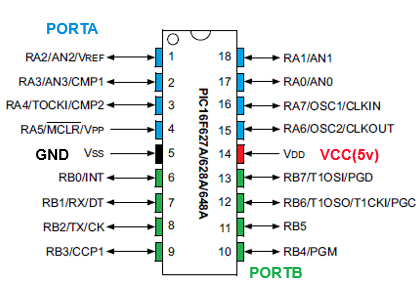
\includegraphics[width=0.85\textwidth]{imgs/cap_3/PIC16F68a_pinout.png}
  \caption{Pinagem do PIC16F628A}
  \label{fig:pic16f628a_pinout}
\end{figure}
\begin{itemize}
    \item \textbf{PORTA (Pinos Azuis):} 
    \begin{itemize}
        \item Pinos 1-4, 17-18 - Porta bidirecional de I/O
        \item Capacidade de entrada analógica \textbf{(AN0-AN3)}
        \item Funções especiais como comparadores, masterclear e entre outros.
        \item Oscilador externo \textbf{(RA6-RA7)} nos pinos 16-17
    \end{itemize}
    
    \item \textbf{PORTB (Pinos Verdes):} 
    \begin{itemize}
        \item Pinos 6-13 - Porta bidirecional de I/O digital
        \item Comunicação serial \textbf{(TX-RX)}
        \item Interrupção externa \textbf{(INT)}
        \item Módulo CCP \textbf{(Capture/Compare/PWM)}
        \item Gravação de programa \textbf{PGD, PGC e PGM}
    \end{itemize}
    
    \item \textbf{Alimentação:} 
    \begin{itemize}
        \item VSS (Pino 5) - Terra \textbf{(GND)}
        \item VDD (Pino 14) - Alimentação positiva \textbf{(5V)}
    \end{itemize}
\end{itemize}

\section{Organização de Memória}
O microcontrolador PIC16F628A possui uma arquitetura de memória Harvard modificada, com separação física entre memória de programa e dados. Sua organização de memória é crucial para entender seu funcionamento e programação.
\subsection{Memórias}
\begin{itemize}
    \item \textbf{Memória de Programa (Flash):} A memória de programa do PIC16F628A é do tipo Flash, permitindo reprogramação elétrica e é o local onde fica armazenado a progração do PIC.
    \item \textbf{Memória de Dados (RAM):} A memória de dados do PIC16F628A é organizada em bancos, banco 0 e banco 1, a RAM é classificada em dois tipos:
    \begin{itemize}
        \item \textbf{SFR (Registradores de Funções Especiais):} Controlam o funcionamento do dispositivo.
        \item \textbf{GPR (Registradores de Propósito Geral):} Para armazenamento de dados do temporários.
    \end{itemize}
    \item \textbf{EEPROM de Dados:} É uma memória não-volátil presente no PIC16F628A que tem a função de armazenar dados permanentes que precisam ser mantidos mesmo quando o dispositivo é desligado.
    \item \textbf{Memória de Configuração:} É uma área especial da memória de programa (Flash) que define o comportamento fundamental do microcontrolador armazenando os bits de configuração.
\end{itemize}
\subsection{Principais Registradores}
\begin{table}[H]
  \centering
  \begin{tabular}{|c|c|c|}
  \hline
  \textbf{Registrador} & \textbf{Função} & \textbf{Endereço} \\
  \hline
  STATUS & Status da ALU e seleção de banco & 0x03 \\
  \hline
  TRIS & Direção dos pinos do PORTB & 0x86 \\
  \hline
  PORT & Estado dos pinos de I/O & 0x06 \\
  \hline
  INTCON & Controle de interrupções & 0x0B \\
  \hline
  \end{tabular}
  \caption{Registradores Especiais por Banco}
  \label{tab:bancos_memoria}
\end{table}

\chapter{Configurações de IDE e Projeto}
\section{Ferramentas Necessárias}
Para a começarmos a programar em PICs, precisaremos assim como no Arduino utilizar uma IDE compatível, nesse caso a fabricante tem seu próprio ambiente de desenvolvimento o MPLAB-X da Microchip e juntamente com ele precisaremos escolher um compilador para programar no caso vamos usar um de 8 bits padrão para que possamos programar em C e utilizaremos o compilador XC8 também da Microchip. Os links para download estão abaixo:
\begin{itemize}
  \item MPLAB-X IDE: \url{https://www.microchip.com/en-us/tools-resources/develop/mplab-x-ide}
  \item XC8 C Compiler: \url{https://www.microchip.com/en-us/tools-resources/develop/mplab-xc-compilers/downloads-documentation#XC8}
\end{itemize}
Faça o download das ferramentas de acordo com o seu sistema operacional, depois disso instale conforme recomenda o fabricante.
Ao iniciar o MPLAB X pela primeira vez, será solicitado que você selecione o diretório que será salvo os programas.

\section{Criação de Projeto}
O MPLAB X IDE organiza todo o desenvolvimento dentro de projetos, que agrupam códigos-fonte, arquivos de cabeçalho e configurações, iremos usar o modelo \textbf{PIC16F628A} para criar um novo projeto, siga os passos abaixo:

\begin{enumerate}
    \item Abra o MPLAB X IDE.
    \item Selecione \textbf{File $\rightarrow$ New Project} ou clique no ícone \textbf{Create New Project} na página inicial.
    \item Na aba de novo projeto que aparece, selecione:
    \begin{itemize}
        \item Categories: \textbf{Microchip Embedded}
        \item Projects: \textbf{Application Project(s)}
        \item Clique em \textbf{Next}
    \end{itemize}
    \item Na aba de seleção de dispositivo, selecione:
    \begin{itemize}
        \item Family: \textbf{All Families ou Escolha a família que deseja usar}
        \item Device: \textbf{Escreva o modelo que deseja programar}
         \item Tool: \textbf{Deixe em No tool ou se estiver com o PICkit conectado ao PC selecione o mesmo}
        \item Clique em \textbf{Next}
    \end{itemize}
    \item Em Select Header \textbf{Não Mexa e clique em Next}
    \item Na aba de Select Compiler, selecione o compilador
    \begin{itemize}
        \item \textbf{XC8(versão)}
    \end{itemize}
    \item clique em \textbf{Next}
    \item Na aba Select Project Name, coloque o nome do projeto
    \item Clique em \textbf{Finish} para concluir a criação
\end{enumerate}
\vspace{-2cm}
Abaixo estão algumas imagens do processo:
\vspace{-1cm}
\begin{figure}[ht]
    \centering
    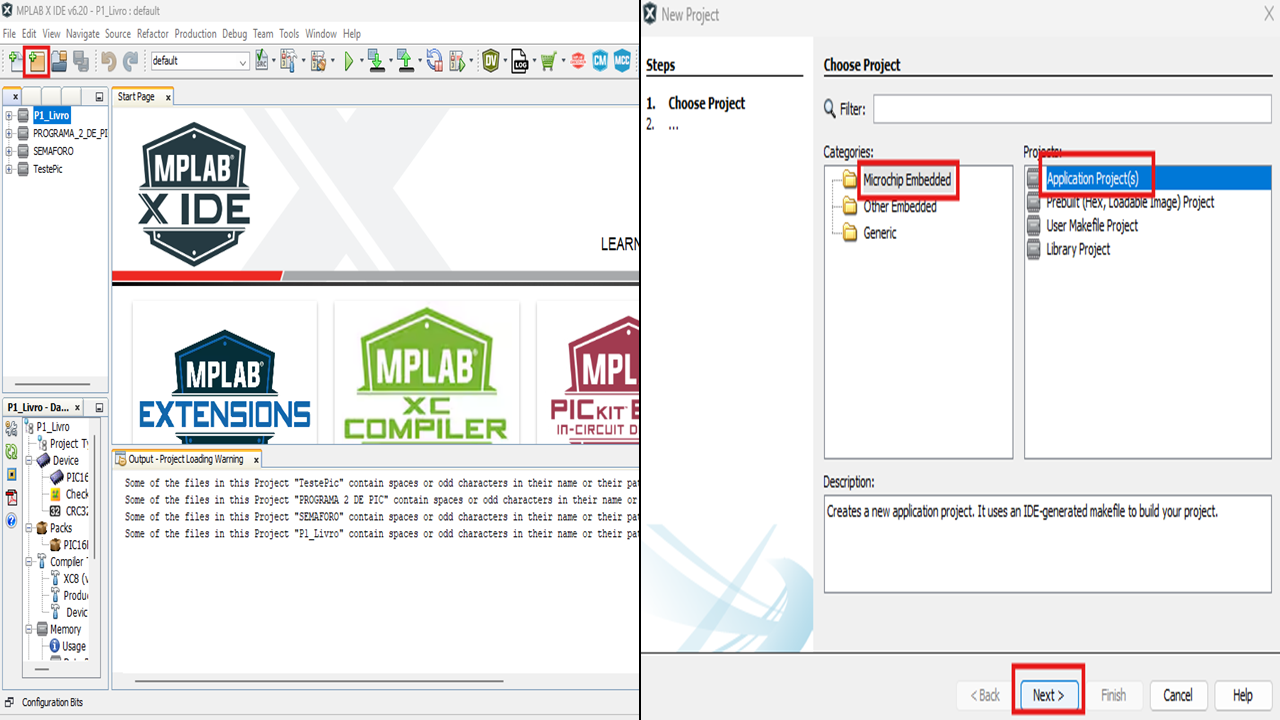
\includegraphics[width=0.8\textwidth]{imgs/cap_4/ide_1.png}
    \caption{Tela de criação de projeto e dispositivo no MPLAB X IDE}
    \label{fig:criar_projeto}
\end{figure}

\begin{figure}[H]
    \centering
    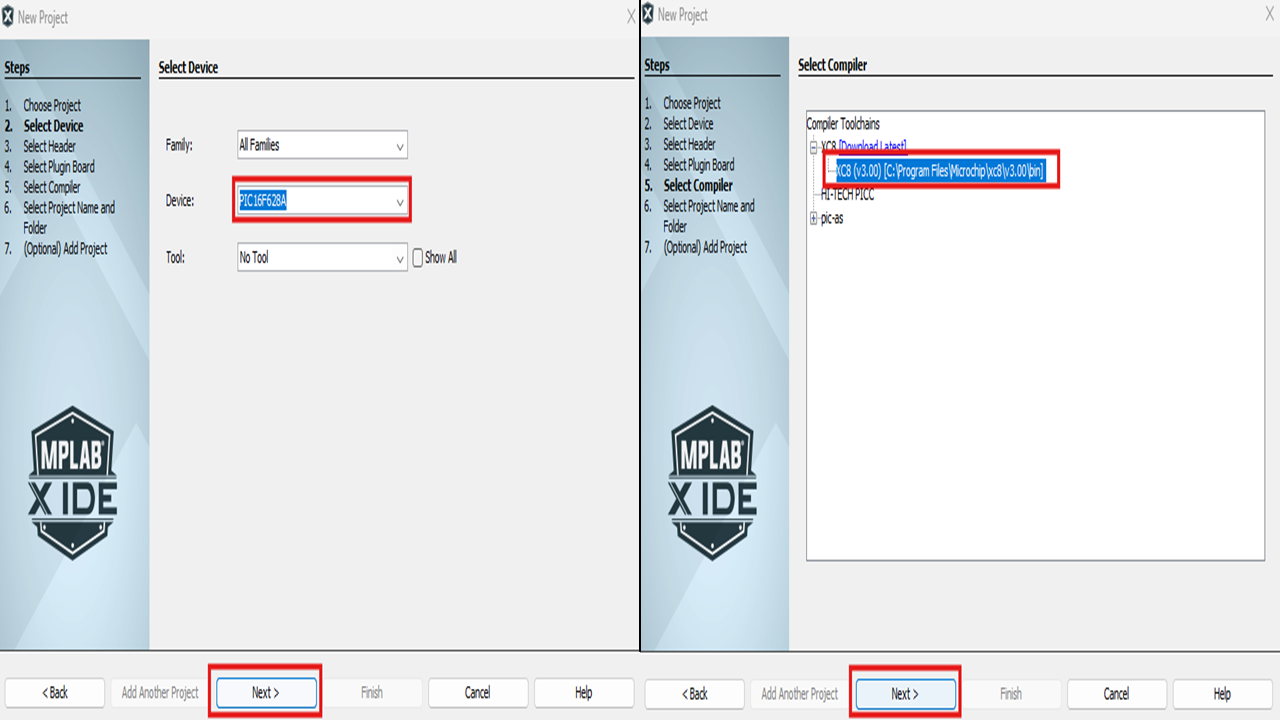
\includegraphics[width=0.8\textwidth]{imgs/cap_4/ide_2.png}
    \caption{Seleção do microcontrolador PIC16F628A e compilador}
    \label{fig:selecao_dispositivo}
\end{figure}
\vspace{-0.5em} % Ajuste fino
Agora com o Projeto criado aba da lateral esquerda na qual tem o nome do projeto maximize-o, clique em  \textbf{Source Files} e com o botão direito nele \textbf{New$\rightarrow$ main.c} que é diferente de \textbf{C Main File} que é para outros compiladores diferentes do \textbf{XC8}.
\subsection{Bits de Configuração do PIC}
Com a \textbf{Main.c} feita, clique em \textbf{Production$\rightarrow$Set Configuration Bits} e nessa etapa você irá configurar o PIC para receber o programa, os \textbf{Configuration Bits} variam entre cada Microcontrolador e após escolher as configurações clique em \textbf{\textit{Generate Source Code to Output}} ele ir gerar uma série de \textbf{pragma configs} que você deve copiar e colar antes dos \textbf{includes} no código.Na aba de Configuration Bits ele da uma pequena explicação do que significa cada configuração, mas em \qty{80}{\percent} as configurações são parecidas mudando um pouco o nome dela contudo mantendo o mesmo funcionamento.A seguir uma explicação de algumas delas:
\begin{itemize}
    \item \textbf{FOSC(Frequency Oscillator):} Responsável pela fonte de frequência que o PIC irá utilizar para sincronizar todas as operações e leituras.
    \begin{itemize}
        \item \textbf{XT:} Utiliza um Cristal externo de média frequência entre 4-20 MHz.
        \item \textbf{HS:} Utiliza um Cristal externo de alta frequência maiores que 8 MHz.
        \item \textbf{EXTRC:} Oscilador externo baseado em Resistor e Capacitor, mas com baixa precisão e estabilidade.
        \item \textbf{INTOSC:} Utiliza um Oscilador interno se o $\mu$C tiver.
        \item \textbf{LP:} Utiliza um Cristal externo de baixa frequência.
    \end{itemize}
     \item \textbf{WDTE(Watch Dog Timer):} Uma medida de segurança que reinicia o PIC ao ser chamado via software ou de forma periódica.
    \begin{itemize}
        \item \textbf{ON}
        \item \textbf{OFF}
        \item \textbf{NSLEEP:} Desligado no modo Sleep.
        \item \textbf{SWTEN:} ON ou OFF de modo dinâmico via software.
    \end{itemize}
    \item \textbf{PWRTE(Power-Up Timer):} Garante a estabilidade de tensão, atrasando a inicialização, recomendável para fontes de tensão instáveis.
    \begin{itemize}
        \item \textbf{ON:} Verifica se tensão está estável.
        \item \textbf{OFF}
    \end{itemize}
    \item \textbf{BOREN (Brown-Out):} Reinicia o $\mu$C se a tensão estiver abaixo de um limite programado.
    \begin{itemize}
        \item \textbf{ON:} Se ligado junto com \textbf{PWRTE} ele espera a estabilidade de tensão primeiro.
        \item \textbf{OFF}
    \end{itemize}
    \item \textbf{LVP(Low Voltage Programming):} Habilita o $\mu$C a programar em tensão de \textbf{3.3v} (requer um circuito específico).
    \begin{itemize}
        \item \textbf{ON}
        \item \textbf{OFF}
    \end{itemize}
    \item \textbf{CPD(Code Protection Data):} Protege a leitura e cópia dos dados armazenados na \textbf{EEPROM}.
    \item \textbf{CP(Code Protection):} Protege a leitura  dos dados armazenados na \textbf{Memória Flash}.

    \textcolor{blue}{CPs podem ser ON ou OFF}
    \item \textbf{WRT(Write Protection):} Protege os dados da \textbf{Memória Flash} evitando reescrita de dados após a inicialização do programa.
    \begin{itemize}
        \item \textbf{256:} Últimos 256 bits 
        \item \textbf{Half:} Metade de baixo
        \item \textbf{Upper Half:} Metade de cima
        \item \textbf{Quarter ou 1/4:} \qty{25}{\percent} do programa.
    \end{itemize}
\end{itemize}
\vspace{-1cm}
\begin{tcolorbox}[
    enhanced,
    title={\textbf{\textcolor{white}{ATENÇÃO}}},
    colback=red!5!white,
    colframe=red!75!black,
    fonttitle=\bfseries\large,
    colbacktitle=red!85!black,
    coltitle=white,
    arc=4pt,
    boxrule=2pt,
    top=8pt,
    bottom=8pt,
    left=8pt,
    right=8pt,
    overlay={
        \node[anchor=north east] at (frame.north east) 
        {
\includegraphics[width=20mm]{imgs/cap_4/warning-icon-svg-27.jpg}};
    }
]
\begin{itemize}[noitemsep,leftmargin=2em]
    \item Ativar \texttt{CP}, \texttt{CPD} ou \texttt{WRT} bloqueia permanentemente:
    \begin{itemize}[noitemsep,leftmargin=3em]
        \item Leitura do firmware (engenharia reversa)
        \item Regravação do microcontrolador
    \end{itemize}
    
    \item \textbf{Nunca} habilite estas opções durante o desenvolvimento
    \item Em produção, verifique 3x o código antes de ativar as proteções
    \item PICs protegidos \textbf{não podem ser reescritos e recuperados}
\end{itemize}
\end{tcolorbox}
\subsection{Configurações de Clock}
Seguindo nas configurações básicas do PIC, no código depois dos \textbf{includes} se deve definir um valor para o \textbf{\textit{Cristal}}
\begin{itemize}
\item \textbf{Padrão}: Se nenhum \texttt{\#pragma config FOSC} for feita, o PIC16F628A utiliza o oscilador interno de \qty{4}{\mega\hertz} (\texttt{INTOSC}) por padrão.
\item \textbf{Comando Universal}: O comando \texttt{\#define \_XTAL\_FREQ} deve ser usado \textbf{sempre}, independentemente do tipo de oscilador e se não utilizado o valor padrão do Cristal será \qty{4}{\mega\hertz}. 
\end{itemize}
\chapter{Programação Prática de PIC}
\section{GPIO e Gerenciamento de Portas}
Os registradores \textbf{TRIS} (Tri-State) e \textbf{PORT} são fundamentais para o controle de I/O nos PICs:

\begin{itemize}
    \item \textbf{TRISx (Data Direction Register)}:
    \begin{itemize}
        \item Determina se os pinos são entradas (1) ou saídas (0)
    \end{itemize}
    \item \textbf{PORTx (Data Latch Register)}:
    \begin{itemize}
        \item Lê ou Escreve o estado lógico dos pinos se dado pino(s) começão ligados ou desligados
        \item Podemos também com o comando \texttt{PORTxbits.RxN} específicar o pino que estamos utilizando
    \end{itemize}
\end{itemize}
\begin{tcolorbox}[
    enhanced,
    title={\textbf{\textcolor{white}{Boas Práticas}}},
    colback=gray!5!white,
    colframe=gray!75!black,
    fonttitle=\bfseries\large,
    colbacktitle=gray!85!black,
    coltitle=white,
    arc=4pt,
    boxrule=2pt,
    top=8pt,
    bottom=8pt,
    left=8pt,
    right=8pt,
]
Ao contrário de algumas abstrações do Arduino, os Microcontroladores permitem manipulação direta de registradores usando diferentes bases numéricas podendo o programador escolher a que deseja utilizar entre decimal, binário ou hexadecimal.

Tanto o \texttt{TRIS} quanto o \texttt{PORT} podem ser definidos usando binários(exemplo: $=$ 0b0), decimais(exemplo $=$ 0) e hexadecimais(0x00) cabe então você escolher o melhor para dado uso, por exemplo, para definir um conjunto de \texttt{TRIS} diferentes podemos usar binário e definir então se são entradas ou saídas (0b01001011)

\texttt{OBS:} A ordem de leitura quando se define um conjunto é no formato decrescente e sempre configure os registradores \texttt{TRIS} antes de usar \texttt{PORT} para evitar estados flutuantes nos pinos.
\end{tcolorbox}
\subsection{Escrita do Código}
Vamos então abaixo escrever um código simples que irá piscar um \textbf{LED} em uma quantidade x de tempo.
\begin{lstlisting}[language=C, caption=Programa para piscar LED no PIC16F628A, label=code:led_blink]
/*
 * File:   main.c
 * Author: gabriel
 */

// CONFIG
#pragma config FOSC = INTOSCIO  // Oscillator interno
#pragma config WDTE = OFF       // Watchdog desativado
#pragma config PWRTE = OFF      // Power-up Timer desativado
#pragma config MCLRE = ON       // MCLR ativo
#pragma config BOREN = OFF      // Brown-out Reset OFF
#pragma config LVP = OFF        // Low Voltage Prog. OFF
#pragma config CPD = OFF        // Protecao de dados OFF
#pragma config CP = OFF         // Protecao de codigo OFF

#include <xc.h>

#define _XTAL_FREQ 4000000      // Frequencia de 4MHz
#define LED PORTAbits.RA1       // LED conectado em RA1

void main(void) {
    TRISA = 0;            // Todos os pinos PORTA como saida
    PORTA = 0x00;         // Inicializa PORTA em LOW

    while(1) {
        LED = 1;                // Liga LED
        __delay_ms(500);        // Espera 500ms
        LED = 0;                // Desliga LED
        __delay_ms(500);        // Espera 500ms
    }
}
\end{lstlisting}
\subsection{Montagem de Circuito}
Nessa seção trataremos da montagem de circuito, com base no código anterior precisaremos tente montar o circuito antes de olhar o diagrama dos seguintes componentes:
\begin{itemize}
    \item \textbf{Componentes necessários}:
    \begin{itemize}
        \item PIC16F628A
        \item LED (qualquer cor)
        \item Resistor (para o LED)
        \item Resistor (para o MCLR)
        \item Botão (para reset)
        \item Fonte de alimentação $5V$
    \end{itemize}

    \item \textbf{Esquemático}:
    \begin{itemize}
        \item Conecte o LED entre RA1 e GND com resistor
        \item Alimentação: $V_{DD}$ (pino 14) em $5V$, $V_{SS}$ (pino 5) em GND
        \item MCLR (pino 4): Resistor para $V_{DD}$ e botão para GND
        \item Oscilador: Nenhum componente externo necessário (configuração INTOSCIO)
    \end{itemize}
\end{itemize}

Abaixo está o circuito montado no simulador \textbf{Proteus}:
\begin{tcolorbox}[
    enhanced,
    title={},
    colback=white!0,  % Fundo quase branco
    colframe=white!0,       % Moldura cinza
    arc=0pt,
    boxrule=-1pt,
    top=2pt,    % Reduz espaço superior
    bottom=2pt, % Reduz espaço inferior
    left=4pt,
    right=4pt,
    boxsep=0pt, % Elimina espaço interno extra
    before skip=5pt, % Espaço antes da caixa
    after skip=5pt,  % Espaço depois da caixa
    float=!htb, % Controle de posicionamento
    width=\textwidth
]
\centering
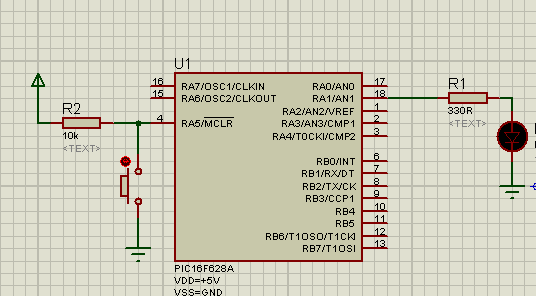
\includegraphics[width=0.85\textwidth]{imgs/cap_4/proj_1.png}
\label{fig:circuito_pisca_led}

\smallskip
\fbox{\parbox{\textwidth\fboxsep-2\fboxrule}{%
    \textbf{Importante:} É sempre necessário ter o \texttt{MCLR} montado corretamente, ele tem a mesma função que o botão reset do Arduino.
}}
\end{tcolorbox}
\newpage
\section{Gravação do PIC}
\subsection{Ferramentas Necessárias}
\begin{itemize}
    \item \textbf{PICkit (Gravador)}: Dispositivo físico para comunicação entre computador e microcontrolador. Modelos recomendados:
    \begin{itemize}
        \item PICkit 3 (suporte até PIC32)
        \item PICkit 5 (modelo mais avançado até o momento)
    \end{itemize}
    \item \textbf{Gravador USB K150:} Uma alternativa ao PICkit para mais informações acesse, \url{www.makerhero.com/blog/como-utilizar-gravador-de-pic-usb-k150/}
    \item \textbf{Soquete ZIF}: Facilita a gravação do PIC
    
\end{itemize}

\subsection{Processo de Gravação com Soquete ZIF}
\begin{enumerate}
    \item Conectar o PICkit ao computador via USB
    \item Inserir o microcontrolador no soquete ZIF:
    \begin{itemize}
        \item Baixar alavanca para destravar o Soquete antes de inserir
        \item A quantidade de pinos do PIC vai definir a sua posição no soquete, no PIC terá um círculo no canto superior esquerdo que indica a posição correta a ser colocada no soquete sempre para cima
        \item Coloque o PIC sempre entre as linhas brancas que estão na parte de trás do soquete
        \item Levantar alavanca para travar após posicionamento do PIC
        \item Vire o soquete e perceba que nele terá marcações \textbf{J1, J2 e J3} que demonstra a posição que está o PIC e na parte de baixo dele o \textbf{DIP} que indicam a quantidade de pinos do $\mu$C e mais abaixo dele tem um conjunto de letras \textbf{J} que serão as configurações.
        \item Volte para frente e coloque as configurações de \textbf{J} inferior vistas atrás do ZIF no \textbf{J} da parte superior respectiva
    \end{itemize}
    
    \item Ligue o PICkit ao ZIF observe atras e conecte corretamente, a seta que aponta para baixo no PICkit indica o \textbf{MCLR(Masterclear)}
    \item Executar gravação na tela da IDE na opção \textbf{Make and program Device Main Project}
    \item \textbf{Em caso de ERRO de VDD na hora da gravação:}
    \begin{itemize}
        \item Na IDE clique no canto superior esquerdo em \textbf{File} $\rightarrow$ \textbf{Project Properties}
        \item No menu que abrir na lateral esquerda vá em \textbf{PICkit} $\rightarrow$ \textbf{Option categories}, selecione \textbf{Power}
        \item Nas opções de \textbf{Power} marque a primeira caixa e na opção de \textbf{Voltage Level} coloque \textbf{4.625}
        \item Aplique as configurações e tente gravar novamente
    \end{itemize}
\end{enumerate}

\begin{figure}[h]
    \centering
    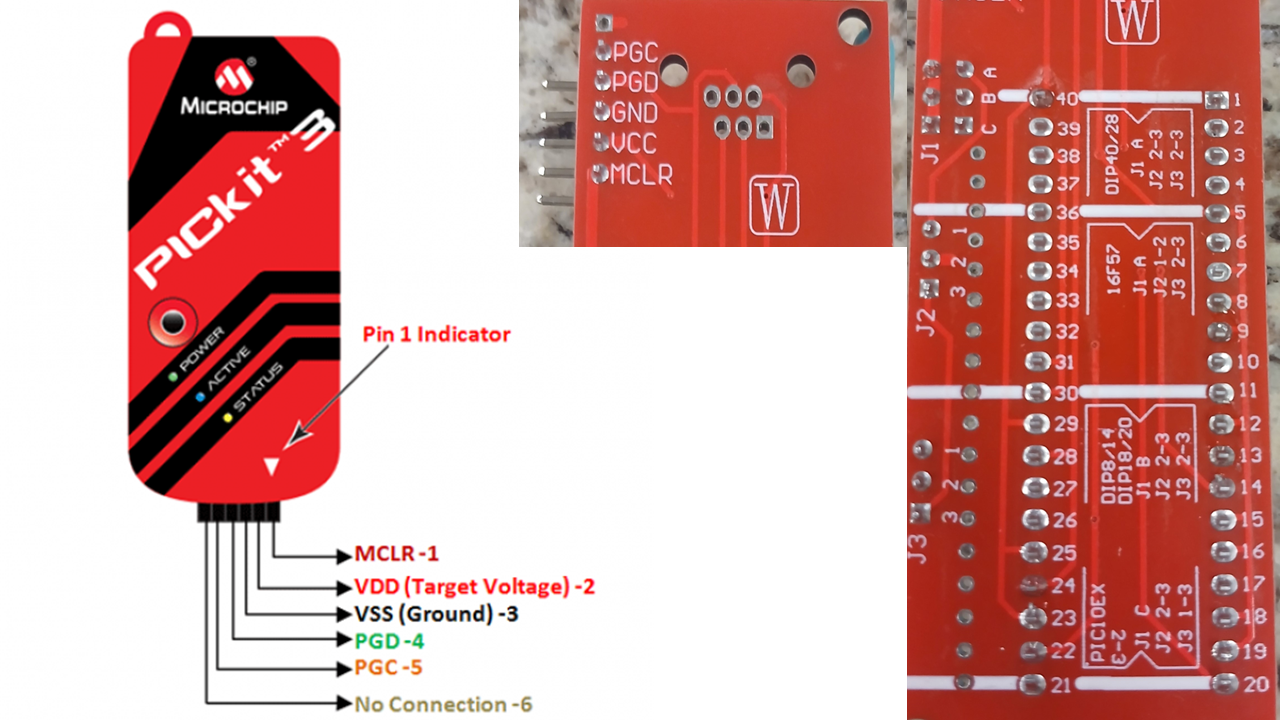
\includegraphics[width=0.9\textwidth]{imgs/cap_4/pickit_soquete.png}
    \caption{Conexão PICkit 3 com soquete ZIF}
    \label{fig:pickit_connection}
\end{figure}
Após tudo isso o circuito do \textbf{PISCA LED} já deve estar funcionando e o \textbf{LED} piscando a meio segundo ou 500 ms.
\begin{tcolorbox}[
    enhanced,
    title={\textbf{\textcolor{white}{ATENÇÃO}}},
    colback=red!5!white,
    colframe=red!75!black,
    fonttitle=\bfseries\large,
    colbacktitle=red!85!black,
    coltitle=white,
    arc=4pt,
    boxrule=2pt,
    top=8pt,
    bottom=8pt,
    left=8pt,
    right=8pt,
    overlay={
        \node[anchor=north east] at (frame.north east) 
        {
\includegraphics[width=10mm]{imgs/cap_4/warning-icon-svg-27.jpg}};
    }
]
\begin{itemize}[noitemsep,leftmargin=2em]
    \item Nunca force o PIC no soquete ZIF, danifica os pinos
    \item Se o PIC já estiver soldado na placa ainda podemos gravar novamente, contanto que não esteja travado a regravação, sem o uso do ZIF utilizando as portas equivalentes diretamente no PIC
\end{itemize}
\end{tcolorbox}
\newpage
\section{Montagem do Cristal}
Ao invés de se utilizar o \textbf{Oscilador Interno} do PIC, podemos montar um circuito com \textbf{Cristal} que é uma fonte de frequência mais precisa do que o interno do PIC, para a montagem podemos olhar no \textbf{datasheet}, pois lá se tem as informações todas as informações que se necessita até mesmo a montagem do Cristal.

Vamos precisar dos seguintes componentes:
\begin{itemize}
    \item \textbf{Capacitores:} Dois capacitores, cada $\mu$C tem seu próprio valor mas os principais são:
    \begin{itemize}
        \item \textbf{22 F ou 22 (real)}
        \item \textbf{33 F ou 33 (real)}
    \end{itemize}
    \item \textbf{Cristal:} Um cristal de qualquer frequência desde que o especifique no código do programa
\end{itemize}
Passos para a Montagem:
\begin{enumerate}
    \item Conecte cada capacitor a um terminal do \textbf{Cristal}
    \item Conecte a outro extremidade do cristal as portas \textbf{CLKIN} e \textbf{CLKOUT} do microcontrolador
    \item Conecte a outra extremidade dos capacitores ao \textbf{GND}
    \item Especifique no código a frequência do cristal
\end{enumerate}
Abaixo esta o diagrama da montagem:
\begin{figure}[h]
    \centering
    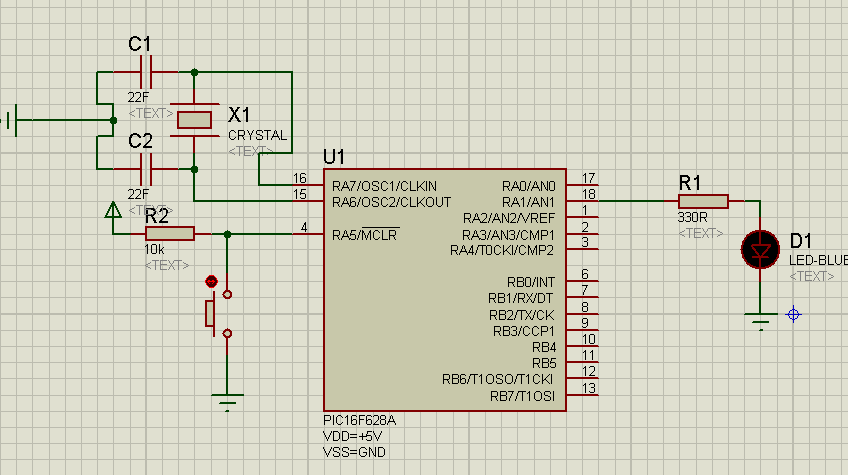
\includegraphics[width=0.9\textwidth]{imgs/cap_5/cristal_pic.png}
    \caption{Montagem do Cristal}
    \label{fig:diag_cristal}
\end{figure}

\chapter{Módulos do PIC16}
\section{Timers e Interrupções}
\subsection{Timers}
Os \textbf{Timers} são módulos internos do microcontrolador que contam \textbf{Pulsos de Clock ou Eventos Externos}, divididos em contadores que contam algum evento e temporizadores que contam intervalos de tempo, ambos não precisam bloquear a execução do programa diferente do comando \texttt{\_\_delay\_ms()}, os Timers são amplamente utilizado em sistemas em tempo real, ao chegar ao seu valor máximo ou a um valor pré-determinado assim como em \textbf{Displays} ele estoura (\textbf{Overflow}) e volta a contagem para zero, podendo nesse momento de \textbf{Estouro} acionar uma interrupção ou mecanismo. Em geral tirando alguns modelos em específico os \textbf{PICs} de 8-bits padrão possuem a mesma quantidade de timers, são eles:
\begin{itemize}
    \item \textbf{Timer0:} É um timer de 8 bits simples, amplamente usado para delays curtos, eventos simples ou interrupções de baixa prioridade tendo somente o \textbf{Prescaler}.
    \begin{itemize}
        \item Pode ser configurado usando o comando \textbf{TMR0} que conta de 0 a 255
        \item Pode ser incrementado por fontes internas usando o \textbf{Clock Interno} com cálculo do $FOSC / 4$ ou incrementado por fontes externas dependendo da configuração do $OPTION\_REG$
    \end{itemize}
    \item \textbf{Timer1:} É timer de 16 bits usado para contagens maiores e intervalos de tempo mais longos ou maior precisão
    \begin{itemize}
        \item Divido em 2 registradores que formam 16 bits com comandos  \textbf{TMR1H} e \textbf{TMR1L} que contam até 65.535
        \item Pode funcionar em modo \textbf{Timer} que incrementa com o clock interno ou em modo \textbf{Count} que conta pulsos externos
        \item Pode ser configurado com o comando \textbf{T1CON}
    \end{itemize}
    \item \textbf{Timer2:} É um timer de 8 bits com recursos de \textbf{prescaler}, divide a frequência antes do clock interno, e \textbf{postscaler}, divide a frequência do evento/interrupção, utilizados para gerar uma contagem mais precisa a partir de um valor definido ou aplicações com \textbf{PWM}
    \begin{itemize}
        \item Pode ser utilizado com o comando \textbf{TMR2} que vai fazer a contagem e o comando \textbf{PR2} que define o período
        \item Quando \textbf{TMR2} atinge o valor definido em \textbf{PR2}, ele reinicia e pode acionar uma interrupção.
    \end{itemize}
\end{itemize}
\subsection{Configuração de Prescaler/Postscaler}
\begin{table}[H]
  \centering
  \begin{tabular}{|c|c|c|c|}
    \hline
    \textbf{PS2} & \textbf{PS1} & \textbf{PS0} & \textbf{Taxa} \\
    \hline
    0 & 0 & 0 & 1:2 \\
    0 & 0 & 1 & 1:4 \\
    0 & 1 & 0 & 1:8 \\
    0 & 1 & 1 & 1:16 \\
    1 & 0 & 0 & 1:32 \\
    1 & 0 & 1 & 1:64 \\
    1 & 1 & 0 & 1:128 \\
    1 & 1 & 1 & 1:256 \\
    \hline
  \end{tabular}
  \caption{Prescaler do Timer0 (OPTION\_REG)}
\end{table}

\begin{table}[H]
  \centering
  \begin{tabular}{|c|c|c|c|}
    \hline
    \textbf{Prescaler} & \textbf{Taxa} & \textbf{Postscaler} & \textbf{Taxa} \\
    \hline
    00 & 1:1 & 0000 & 1:1 \\
    01 & 1:4 & 0001 & 1:2 \\
    1x & 1:16 & 0010 & 1:3 \\
    ... & ... & ... & ... \\
    ... & ... & 1111 & 1:16 \\
    \hline
  \end{tabular}
  \caption{Prescaler e Postscaler do Timer2 (T2CON)}
\end{table}

\subsection{Interrupções}
Interrupções são mecanismos que permitem que o $\mu$C suspenda a execução de programa para executar uma rotina de tratamento com o comando \textbf{(ISR – Interrupt Service Routine)} em resposta a um evento específico. Essa abordagem possibilita a resposta imediata a eventos externos ou internos, sem a necessidade de \textbf{polling constante (verifica repetidamente se houve uma mudança em um evento)}, microcontroladores \textbf{PIC} de 8-bits não possuem prioridade de interrupções nativa ao contrário de modelos 16/32 bits. 
\paragraph{Tipos de interrupções:}
\begin{itemize}
    \item \textbf{Interrupção Gobal (GIE):} Para que qualquer interrupção seja processada, o bit global de interrupções (GIE) e, geralmente, o bit de interrupções periféricas (PEIE) devem ser configurados para 1.
    \item \textbf{Interrupção Específica (Cada Módulo):} Timer0, Timer1, Timer2, comunicação serial, entrada externa e entre outros módulos possuem seu próprio  comando de \textbf{Interrupt Enable Bit} e de \textbf{Flag}, por exemplo: 
    \begin{itemize}
        \item \textbf{Timer0 (T0IE)} e se a flag foi configurada por \textbf{T0IF} ele executa a ISR
        \item \textbf{Timer1 (TMR1IE)}e se a flag foi configurada por \textbf{TMR1F} ele executa a ISR
        \item \textbf{Timer 2(TMR2IE)}e se a flag foi configurada por \textbf{TMR2IF} ele executa a ISR  .
    \end{itemize}
\end{itemize}
\paragraph{Exemplo de Código:} Gerar uma interrupção e alternar o estado de um LED conectado a um pino
\begin{lstlisting}[language=C, caption=Programa para relogio e LCD no PIC16F628A, label=code:led_blink]
/*
 * File:   main.c
 * Author: gduar
 *
 * Created on 3 de Abril de 2025, 11:02
 */

// CONFIG
#pragma config FOSC = XT // Oscillator Selection bits (INTOSC oscillator: I/O function on RA6/OSC2/CLKOUT pin, I/O function on RA7/OSC1/CLKIN)
#pragma config WDTE = OFF       // Watchdog Timer Enable bit (WDT disabled)
#pragma config PWRTE = OFF      // Power-up Timer Enable bit (PWRT disabled)
#pragma config MCLRE = ON       // RA5/MCLR/VPP Pin Function Select bit (RA5/MCLR/VPP pin function is MCLR)
#pragma config BOREN = OFF      // Brown-out Detect Enable bit (BOD disabled)
#pragma config LVP = OFF        // Low-Voltage Programming Enable bit (RB4/PGM pin has digital I/O function, HV on MCLR must be used for programming)
#pragma config CPD = OFF        // Data EE Memory Code Protection bit (Data memory code protection off)
#pragma config CP = OFF         // Flash Program Memory Code Protection bit (Code protection off)

#include <xc.h>

#define _XTAL_FREQ 4000000
#define LED PORTBbits.RB0

volatile uint8_t temporizador = 0;

volatile struct {
    volatile uint8_t SEG;
    volatile uint8_t MIN;
} relogio = {0, 0};


void main(void) {
    TRISB = 0x00;
    PORTB = 0x00;
    
    iniciar_timer0();
    
    while (1){
    LCD_SetCursor(0,0);
    LCD_Print(relogio.SEG);
    LCD.SetCursor(0,1);
    LCD.Print(relogio.MIN);
    }
}

void __interrupt() isr() {  
    if (INTCONbits.T0IF) {
        temporizador++;
        if(temporizador >= 15){
            relogio.SEG++;  
            temporizador = 0;
        }
        if(relogio.SEG >= 60) {
            relogio.SEG = 0;
            relogio.MIN++;
        }
        TMR0 = 0;            // Ajusta para overflow a cada ~65.5ms  
        INTCONbits.T0IF = 0;  // Limpa flag de interrupção
    }  
}  


void iniciar_timer0() {  
    OPTION_REG = 0b00000111; // Prescaler 1:256, clock interno  
    TMR0 = 0;                // Inicia contagem em 0  
    INTCONbits.T0IE = 1;     // Habilita interrupção do Timer0
    INTCONbits.GIE = 1;      // Habilita interrupções globais  
}
\end{lstlisting}

\section{Comparadores}
Os \textbf{Comparadores Analógicos} são periféricos integrados em \textbf{PICs} que permitem comparar dois sinais analógicos e gerar uma saída digital indicando qual sinal é maior. Eles são utilizados em aplicações que envolvem sensores analógicos, controle de tensão e conversões analógico-digitais simplificadas. O \textbf{PIC16F628A} contém 2 comparadores que estão presentes nos pinos \textbf{RA0 a RA3} que pode ser configurado pelo comando \textbf{CMCON (Comparator Module Control Register)}.
\paragraph{Os bits dele podem ser configurados por:}
\begin{itemize}
    \item \textbf{CM2 e CM0:} Seleciona a configuração dos comparadores
    \begin{itemize}
        \item Ambos os comparadores habilitados
        \item Ambos desabilitados
        \item Um comparador habilitado com referência interna (\textbf{VREF})
    \end{itemize}
    
    \item \textbf{CIS:} Alternas as entradas positivas e negativas
    \item \textbf{C1OUT e C2OUT:} Indicador do estado de saída dos comparadores
    \item \textbf{C1INV / C2INV:} Inverte a polaridade da saída
\end{itemize}
\begin{table}[h]
\centering
\begin{tabular}{|c|c|l|}
\hline
\textbf{CM2:CM0} & \textbf{Hex} & \textbf{Modo de Operação} \\
\hline
000 & 0x00 & Comparadores independentes \\
\hline
001 & 0x01 & Três entradas multiplexadas \\
\hline
010 & 0x02 & Comparador com referência interna \\
\hline
100 & 0x04 & Duas entradas comuns (invertidas) \\
\hline
111 & 0x07 & Comparadores desativados (pinos como I/O digitais) \\
\hline
\end{tabular}
\caption{Modos de Operação dos Comparadores (PIC16F628A)}
\label{tab:cmcon_simple}
\end{table}

\paragraph{Modos de Operação:}
\begin{itemize}
    \item \textbf{Independente:} Cada comparador opera de forma separada com entradas diferentes para $V^+$ e $V^-$
    \item \textbf{Referência Comum \textbf{(VREF)}:} Ambos os comparadores compartilham a mesma entrada positiva $V^+$ e independentes $V^-$
\end{itemize}
\section{Comunicação Serial (USART)}
\chapter{Programação Avançada de PIC}
\section{Option Registers}
\section{Status}
\section{Bit Baggin}
\section{Debounce}
\section{Otimização}
Nessa seção trataremos de uma programação
\chapter{Periféricos Essenciais}
\section{LCDs}
\section{Conversor A/D}

\chapter{Projetos Baseados em Problemas}
\subsection{Sistema de Controle}
\subsection{Monitor de Temperatura}
\subsection{Interface Homem-Máquina}


\end{document}